\chapter{Foundations}

	% Intro
	% First part: Transformations
	%	Representation for pose
	% 	Representation for pose in sequences: Figure
	% Second part: Deep Learning
	% Third part: Toy examples for RNN
	This chapter presents the necessary theoretical background for the thesis.
	The first part is about the representation of the camera pose, which is ultimately the output of a system for Visual Odometry.
	In the second part, it follows a very brief review of Deep Learning.
	In particular, the recurrent neural network, an important building block for the Visual Odometry model in this thesis, is introduced.
	For a more comprehensive insight into Deep Learning, the reader is advised to consult \cite{goodfellow2016deep}.
	
	\section{Transforming Camera Pose}
		The camera pose, also known as the \emph{extrinsic parameters}, is a combination of position and orientation.
		Together, they define a coordinate transformation from the camera coordinate frame to the world coordinate frame.
		Such a transformation is commonly represented by a translation vector $\vectr{t} \in \R^3$ and a rotation matrix $\matr{R} \in SO(3)$. 
		Together, they describe a rigid transformation which can also be written as a $4 \times 4$ matrix of the form
		\begin{equation}\label{eq:pose_representation_se3}
			\matr{T} = 
			\begin{bmatrix}
				\matr{R} 	& \vectr{t} \\
				0 			& 1
			\end{bmatrix} 
			\in SE(3).
		\end{equation}
		\todo{Insert a figure showing: world coordinate frame, camera coordinate frame, transformation matrix}
		
		In Structure from Motion (SfM), there is not only one camera, but many cameras with different transformations.
		This is also the case in Visual Odometry (VO), but the sequence of transformations is ordered according to the path of the camera motion. 
		Specifically, we deal with a sequence of rotations $\matr{R}_1, \dots, \matr{R}_n$ and translations $\vectr{t}_1, \dots, \vectr{t}_n$. 
		Depending on how the poses are obtained, they are all relative to a common (world) coordinate frame.
		Sometimes it is necessary or useful to have all transformations relative to a new coordinate system.
		This can be achieved by applying the transformations
		\begin{align}\label{eq:relative_rotation_conversion_general}
			\begin{split}
				\matr{R}_{i \rightarrow j} 		&= \matr{R}_{j}^{\top} \matr{R}_{i} \\
				\vectr{t}_{i \rightarrow j} 	&= \matr{R}_{j}^{\top} (\vectr{t}_i - \vectr{t}_j)
			\end{split}
		\end{align}
		to get the new relative rotation 
		$\matr{R}_{i \rightarrow j}$ and relative translation $\vectr{t}_{i \rightarrow j}$.
		The arrow notation $i \rightarrow j$ denotes that the $i$-th transformation is in coordinates of system $j$.
		Note that for $i = j$ we obtain 
		$\matr{R}_{i \rightarrow j} = \matr{I}$ 
		and 
		$\vectr{t}_{i \rightarrow j} = \vectr{0}$.
		
		The formulas in equation~\ref{eq:relative_rotation_conversion_general} can be applied to every transformation in the sequence for $i = 1, \dots, n$ and having $j$ fixed, e.g.\@ $j = 1$ would make all transformations relative to the first camera coordinate system.
		In the remainder of this thesis we refer to the camera pose in this format as the \emph{global pose}, where the first pose in the sequence always represents the coordinate system of all other poses.
		An alternative choice is $j = i - 1$.
		We refer to this special setting as the \emph{incremental pose}, since all transformations are relative to the previous video frame, i.e.\@ we have 
		$\matr{R}_{i \rightarrow i - 1}$ and $\vectr{t}_{i \rightarrow i - 1}$
		for $i = 2, \dots, n$.
		
	\section{Representations for Pose}
		
		So far, we have seen the camera pose represented as a $4 \times 4$ transformation matrix with a rotational and translational part (equation~\ref{eq:pose_representation_se3}).
		In a system for VO we could, for example, aim to compute the rotation and translation separately and then plug them together into a transformation matrix.
		For the translation, the system would need to estimate the three components in X-, Y- and Z-direction.
		However, it is unclear how the system should be designed to output the elements of a rotation matrix, since it is constrained to be in 
		$SO(3)$, which is the group of matrices with determinant equal to one and for which the transpose is equal to the inverse.
		%$SO(3) = \lbrace \matr{A} \in \R^{3 \times 3} \mid \matr{A}^{-1} = \matr{A}^\top \land \det(\matr{A}) = 1 \rbrace$.
		A constraint like this is difficult to enforce directly.
		
		Actually, it is redundant to describe rotations with nine numbers when in fact there are only three degrees of freedom for a rotation in 3D, i.e., two degrees are needed for the orientation of the axis and one for the angle of rotation around the axis.
		It is also not straightforward to interpolate rotations in $SO(3)$, or to find the best approximation for a matrix that lies outside of $SO(3)$.
		The later is definitely useful when numerical errors occur in computations involving the rotation.
		
		What follows is a discussion and comparison of three other popular representations used to describe rotations.
		A brief overview is also shown in table~\ref{tbl:comparison_representations_of_rotations}.
		\begin{table}
			\small
			\begin{center}
				\begin{tabular}{llll}
					% Typical use case & Robotics, Avionics & Computer Graphics, Physics & Intermediate representation & Computer Graphics,
					\toprule
					Representation	& Constraint 			& Problems 				& Identity			\\
					\midrule
					Euler angles 	& None 					& Gimbal lock 			& ambiguous 		\\
					Axis-angle 		& Unit-norm axis 		& Missing algebraic structure						& ambiguous 		\\
					Matrix 			& Must be in $SO(3)$ 	& Numerical instability	& unique 			\\
					Unit quaternion & 4D unit sphere 		& Less intuitive 		& unique			\\
					\bottomrule
				\end{tabular}
			\end{center}
			\caption[A comparison of representations for rotations]
					{A comparison of representations for rotations.
					 \label{tbl:comparison_representations_of_rotations}}
		\end{table}
	
		\paragraph{Euler Angles}
%		The fact that rotations in 3D have three degrees of freedom means there are only three coordinates needed to identify a rotation. 
%		Euler angles are one such choice of coordinates.
		The Euler angles represent a rotation with three numbers 
		$\alpha, \beta, \gamma \in \left[0, 2\pi\right)$, which are also known as \emph{pitch}, \emph{roll} and \emph{yaw}.
		There are many different conventions and definitions of these three angles and how they are applied.
		In this thesis, we apply the rotations in the following order. 
		The initial canonical coordinate frame shall be denoted by $(x, y, z)$.
		\begin{enumerate}
			\item The coordinate frame is rotated around the $x$-axis with angle $\alpha$. 
			This results in a new coordinate frame $(x^\prime, y^\prime, z^\prime)$.
			\item Next, the system is rotated around the $y^\prime$-axis by angle $\beta$. 
			The new coordinate frame is $(x^{\prime\prime}, y^{\prime\prime}, z^{\prime\prime})$.
			\item Finally, we perform a rotation around axis $z^{\prime\prime}$ by angle $\gamma$ to obtain the desired orientation.
		\end{enumerate}
		Altogether these steps can be formalized by a multiplication of three matrices that define the rotations around the different axes. 
		The result is a rotation matrix
		\begin{equation}\label{eq:euler_angles_rotation_matrix_arbitrary_axis}
			\matr{R}(\alpha, \beta, \gamma) =
			\matr{R}_{z^{\prime\prime}}^\gamma
			\matr{R}_{y^\prime}^\beta
			\matr{R}_{x}^\alpha
		\end{equation}
		defined by the Euler angles. 
		Although the above description of how the rotations are applied is more or less intuitive, the computation of rotation matrices around arbitrary axes in equation~\ref{eq:euler_angles_rotation_matrix_arbitrary_axis} is a bit complicated.
		Fortunately, it can be shown that 
		\begin{equation}\label{eq:euler_angles_rotation_matrix_global_axis}
			\matr{R}(\alpha, \beta, \gamma) =
			\matr{R}_{x}^\alpha \,
			\matr{R}_{y}^\beta \,
			\matr{R}_{z}^\gamma,
		\end{equation}
		where 
		\begin{align}
			\begin{split}
				\matr{R}_{x}^\alpha &= 
				\begin{bmatrix}
					1 & 0 				& 0 			\\
					0 & \cos(\alpha) 	& -\sin(\alpha) \\
					0 & \sin(\alpha) 	& \cos(\alpha)
				\end{bmatrix}
				\\
				\matr{R}_{y}^\beta &= 
				\begin{bmatrix}
					\cos(\beta) 	& 0 	& \sin(\beta) 	\\
					0 				& 1 	& 0 			\\
					-\sin(\beta) 	& 0 	& \cos(\beta)
				\end{bmatrix}
				\\
				\matr{R}_{z}^\gamma &=  
				\begin{bmatrix}
					\cos(\gamma) 	& -\sin(\gamma) 	& 0 \\
					\sin(\gamma) 	& \cos(\gamma) 		& 0 \\
					0 				& 0 				& 1 
				\end{bmatrix}
			\end{split}
		\end{align}
		are simple rotations around the axes of the initial (canonical) coordinate system $(x, y, z)$.
		Further, it can be shown that this representation covers all 3D rotations, and in reverse, every rotation matrix $\matr{R} \in SO(3)$ can be decomposed into the form in equation~\ref{eq:euler_angles_rotation_matrix_global_axis}, e.g.\@ to extract the Euler angles.
		
		Unfortunately, the Euler angle representation comes with some limitations.
		There are special configurations of angles that can lead to a loss in the degrees of freedom for the rotation. 
		For example, if we fix $\beta = \frac{\pi}{2}$, any choice of values for the other angles results in a matrix where the first row is always the same.
		Therefore, one degree of freedom for rotation is lost.
		This unavoidable problem is also known as \emph{gimbal lock} and it is inherent to the way Euler angles are defined.
		A second limitation worth mentioning is the fact that interpolation between two rotations in Euler form is not intuitive and quite complicated.
		It is better to convert to a different representation and perform the interpolation there, e.g., with quaternions.
		
		\paragraph{Axis-Angle}
		Every rotation in three-dimensional space can be defined by an angle 
		$\theta \in \R$ and a vector 
		$\vectr{a} \in \R^3$ for the axis of rotation.
		We denote it by the tuple $(\vectr{a}, \theta)$.
		The axis can be thought of as the normal vector on the plane in which the rotation takes place.
		The axis itself has three degrees of freedom, but for the rotation, only two of these matter.
		Therefore the axis is often assumed to be normalized, i.e.\@ $\lVert \vectr{a} \rVert = 1$.
		There are two main limitations to the axis-angle, which often make it only usable as an intermediate representation.
		One is the missing algebraic structure to directly concatenate several rotations.
		Second, the representation is ambiguous.
		We have that $(\vectr{a}, \theta)$ represents the same rotation as $(-\vectr{a}, -\theta)$ for all possible axes and angles, and the identity rotation can be represented by any axis-angle $(\vectr{a}, 2 \pi k)$ for $k \in \Z$.
		
		This ambiguity and the unit-norm axis constraint make the axis-angle representation less useful for this work.
		Especially for supervised training of artificial neural networks, it is best to eliminate as many ambiguities as possible to avoid confusion.
		
		\paragraph{Unit Quaternions}
		Quaternions are four-dimensional numbers.
		They are an extension of the complex numbers. %\footnote{A more appropriate name is \emph{compound numbers}.\todo{disputable}}.
		Formally, a quaternion is defined as $\vectr{q} = w + \vectr{i}x + \vectr{j}y + \vectr{k}z$ where $w, x, y, z \in \R$ and $\vectr{i},\vectr{j}$ and $\vectr{k}$ are the basis elements of the quaternion space.
		The quaternion can also be written as a tuple $\vectr{q} = (w, x, y, z) \in \R^4$ by introducing the notation
		\begin{equation}
			\vectr{1} = 
			\begin{bmatrix}
				1 \\ 
				0 \\ 
				0 \\ 
				0
			\end{bmatrix},\quad
			\vectr{i} = 
			\begin{bmatrix}
				0 \\ 
				1 \\ 
				0 \\ 
				0
			\end{bmatrix},\quad
			\vectr{j} = 
			\begin{bmatrix}
				0 \\ 
				0 \\ 
				1 \\ 
				0
			\end{bmatrix},\quad
			\vectr{k} =
			\begin{bmatrix}
				0 \\ 
				0 \\ 
				0 \\ 
				1
			\end{bmatrix}.
		\end{equation}
		But quaternions are not just tuples of numbers. 
		They are equipped with a separate addition and multiplication.
		Addition is simply carried out element-wise as for vectors, whereas multiplication makes use of the distributive rule and the property
		\begin{equation}
			\vectr{i}^2 = \vectr{j}^2 = \vectr{k}^2 = \vectr{i}\vectr{j}\vectr{k} = -\vectr{1}.
		\end{equation}
		Furthermore, the norm of a quaternion is defined as
		\begin{equation}
			\lVert \vectr{q} \rVert = \sqrt{w^2 + x^2 + y^2 + z^2}.
		\end{equation}
		One particularly interesting subset of the quaternions are those with unit norm, i.e., $\lVert \vectr{q} \rVert = 1$.
		They are called \emph{unit quaternions}.
%		In this thesis, we are particularly interested in the subset of quaternions called the \emph{unit quaternions}. These are all the quaternions with unit norm, i.e., $\lVert \vectr{q} \rVert = 1$. 
		The quaternions of this form describe 3D rotations and can be parameterized by
		\begin{equation}
			\vectr{q} = 
			\cos\left(\tfrac{\theta}{2}\right) + 
			\sin\left(\tfrac{\theta}{2}\right) \left(a_1 \vectr{i} + a_2 \vectr{j} + a_3 \vectr{k}\right),
		\end{equation}
		where $\theta \in \R$ is the angle of rotation around a unit-length axis $\vectr{a} = (a_1, a_2, a_3) \in \R^3$.
		The parameterization makes use of the axis-angle representation, however, quaternions are more powerful in the sense that rotations can be concatenated via multiplication, i.e., $\vectr{q}_2 \vectr{q}_1$ represents the compound rotation of $\vectr{q}_1$ followed by $\vectr{q}_2$.
		One drawback of the quaternion is that it is a double cover of the space of rotations, meaning that $\vectr{q}$ and $-\vectr{q}$ represent the same rotation.
		\todo{mention spherical linear interpolation (Slerp)?}
		\\
		
		How well a neural network can be trained to output a rotation may depend on the choice of the representation and its constraints.
		An analysis on this matter is done in chapter~\ref{chp:experiments-and-results}.
		We now continue with a brief review on artificial neural networks and machine learning.
		
	\section{Deep Feedforward Neural Networks}
		
		A \emph{feedforward neural network} is a function mapping an input $\vectr{x}$ to an output $\vectr{y} = f(\vectr{x})$.
		For instance, $\vectr{y} \in \{\text{dog}, \text{cat} \}$ could be the output of the function deciding whether an image $\vectr{x}$ contains a dog or a cat. 
		The reason it is called a \emph{deep network} is because $f$ is often a long chain of function compositions, e.g., 
		$f = f^{(n)} \circ  \ldots  \circ f^{(2)} \circ f^{(1)}$.
		The functions $f^{(1)}, \dots, f^{(n)}$ are called \emph{layers} and $n$ is the \emph{depth} of the network.
		Each layer performs a computation on the output of the previous layer, hence the name \emph{feedforward}.
		\begin{figure}[t]
			\centering
			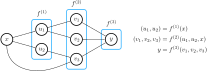
\includegraphics[width=\linewidth]{Foundations/feed-forward-neural-network-example}
			\caption[Example of a feedforward neural network]
					{Example of a feedforward neural network represented by a computational graph. 
					 Each layer (blue) operates on the outputs of previous layers, where $x$ is the input and $y$ is the output.
					 \label{fig:example_feed_forward_network}}
		\end{figure}
		A feedforward network is best visualized as a graph%
		\footnote{More precisely it is a DAG (directed acyclic graph). It does not allow loops.}, 
		the so-called \emph{computational graph}.
		Figure~\ref{fig:example_feed_forward_network} shows an example of a small feedforward network.
		A node in the graph represents an output- or input variable to one of the functions $f^{(i)}$, and the collection of all output nodes for one function is called a \emph{layer}. 
		The edges between nodes represent information flow, i.e., which outputs of layer $j$ depend on the outputs of layer $i$.
		
		Feedforward networks build the foundation of deep learning.
		Why?
		Because in general, $f$ is unknown and must be learned to solve a specific task.
		The practical approach to finding a suitable $f$ is to consider a family of functions $f_{\vectr{w}}$ defined by the \emph{parameters} $\vectr{w}$, also called \emph{weights}.
		For example, the layer $i$ in the network might be a linear function $f_{}^{(i)}(\vectr{x}) = \matr{W} \vectr{x}$ where the parameters of this layer are the elements of the matrix $\matr{W}$.
		
		The collective of all functions in the family is called the \emph{model}.
		To solve the task, e.g., classifying dogs and cats, one has to \emph{train} the model.
		In other words, one has to search through the space of all parameters $\vectr{w}$ to find the ones that perform the best.
		The performance is measured with the \emph{loss function} 
		$\mathcal{L}(f_{\vectr{w}}(\vectr{x}), \vectr{y}) \in \R$ that compares the prediction 
		$\vectr{\hat{y}} = f_{\vectr{w}}(\vectr{x})$ with the \emph{ground truth} $\vectr{y}$ and gives a score how close they are.
		The ground truth comes from the dataset, which is the most important resource of knowledge for training a model.
		The dataset contains many samples $\vectr{x}^{(1)}, \dots, \vectr{x}^{(N)}$ each with a ground truth label 
		$\vectr{y}^{(1)}, \dots, \vectr{y}^{(N)}$, e.g., each dog image in the dataset has a label ``dog" and each image with a cat has the label ``cat".
		
		The loss function is not only used to evaluate the performance of the model, but to find optimal parameters for the model as part of the training.
		In general, the objective is to minimize the loss function on the data, that is
		\begin{equation}\label{eq:optimal_parameter_neural_network}
			\vectr{w}^\ast = \argmin_{\vectr{w}} 
			\sum_{i = 1}^{N} 
				\mathcal{L}(f_{\vectr{w}}(\vectr{x}^{(i)}), \vectr{y}^{(i)}).
		\end{equation}
		The resulting function $f_{\vectr{w}^\ast}$ is a solution that best satisfies the loss function on all the data.
		How can $\vectr{w}^\ast$ be found?
		A common way to minimize the loss is to use gradient descent.
		It is one of the most general purpose optimization algorithms.
		Gradient descent can find a local minimum of a function $F$ by iteratively stepping in the opposite direction of the gradient, which can be described by the update rule
		\begin{equation}
			\vectr{w} \leftarrow 
			\vectr{w} - \lambda \frac{\partial F(\vectr{w})}{\partial \vectr{w}}.
		\end{equation}
		The parameters $\vectr{w}$ approach a local minimum when a suitable learning rate $\lambda$ is chosen.
		In the context of deep learning, $F$ is the loss function evaluated over the training data.
		More precisely, the update rule is
		\begin{equation}\label{eq:gradient_descent_update_rule}
			\vectr{w} \leftarrow 
			\vectr{w} - \lambda 
			\frac{\partial}{\partial \vectr{w}}
			\sum_{i = 1}^{N} 
				\mathcal{L}(f_{\vectr{w}}(\vectr{x}^{(i)}), \vectr{y}^{(i)}).
		\end{equation}
		One parameter update with gradient descent requires the model to be evaluated for the entire dataset.
		This is a very expensive operation and in practice it is most often unfeasible.
		\emph{Stochastic} gradient descent is a modification that performs the update for each sample, which means that the sum in equation~\ref{eq:gradient_descent_update_rule} is dropped and the update rule is simply
		\begin{equation}\label{eq:stochastic_gradient_descent_update_rule}
			\vectr{w} \leftarrow 
			\vectr{w} - \lambda 
			\frac{\partial \mathcal{L}(f_{\vectr{w}}(\vectr{x}^{(i)}), \vectr{y}^{(i)})}{\partial \vectr{w}}.
		\end{equation}
		The following steps describe a typical training procedure of a feedforward network.
		\begin{enumerate}
			\item Define model $f_{\vectr{w}}$
			\item Initialize parameters $\vectr{w}$
			\item Loop over training samples $\vectr{x}^{(i)}$ %for $i = 1, \dots, N$
			\begin{enumerate}
				\item Forward operation: $\vectr{\hat{y}} = f_{\vectr{w}}(\vectr{x}^{(i)})$
				\item Compute loss $\mathcal{L}(\vectr{\hat{y}}, \vectr{y}^{(i)})$
				\item Backward operation: Backpropagate the gradient of the loss 
				\item Update parameters
			\end{enumerate}
		\end{enumerate}
		The algorithm above trains the model using each sample from the dataset once.
		A complete run over the dataset is called one \emph{epoch}.
		To improve the fit of the model to the data further, one can iterate for multiple epochs.
		
		After training it is a good practice to evaluate the model on new data, the test set.
		This way we can measure how well the model generalizes.
		It is important that the model performs well on new data because in practice we are often limited in how much data we can collect for training.
		A model that does not generalize well is not very useful.
		
		Some remarks on the above summary for feedforward neural networks:
		First, training with samples that have a ground truth label is called \emph{supervised learning}.
		It is also possible to learn from data where labels are not available.
		This is called \emph{unsupervised learning}.
		However, the focus of this thesis lies in the supervised approach.
		Second, since the feedforward network is a composition of functions, gradient computation involves the chain rule for differentiation.
		The \emph{backpropagation} algorithm is an efficient implementation for the chain rule that avoids computing the same subexpressions multiple times.
		It is the preferred method to compute gradients in a neural network.
		
	\section{Convolutional Neural Networks}
	
	\section{Recurrent Neural Networks}\label{sec:recurrent_neural_networks}
		\newcommand{\imagecourtesycolah}{Image courtesy Christopher Olah \mbox{\href{http://colah.github.io/}{(colah.github.io)}}.}
		\todo{Need references to early works on RNNs}
		So far, we have looked at the feedforward network, which is a function that maps an input $\vectr{x}$ to an output $\vectr{y} = f(\vectr{x})$.
		It will always compute the same output for the same input, independently of the input-output pairs it has seen before.
		Now consider a sequence $\vectr{x}_1, \dots, \vectr{x}_T$ of inputs, e.g., a sentence.
		How can we learn to predict an attribute that depends on the whole sequence, e.g., the sentiment of the sentence?
		One way is to concatenate the sequence to one vector and use the feed-forward network.
		However, this will limit the sequence length to a fixed size and potentially requires more training data.
		\todo{need reference for this statement}.
		How do we model predictions for a variable sequence length?
		And what if we want also the output to be a sequence? 
		What if the output sequence needs to have a different length than the input sequence, such as in machine translation? 
		\todo{citation needed}
		
		This is where the recurrent neural network (RNN) comes into play.
		It is a function that maps each vector $\vectr{x}_t \in \R^n$ from the sequence to a hidden state
		\begin{eqnarray}
			\vectr{h}_t = R(\vectr{x}_t, \vectr{h}_{t-1}), & &t = 1, \dots, T
		\end{eqnarray}
		with the hidden state $\vectr{h}_{t-1} \in \R^d$ carried over from the previous prediction as a second input, where $d$ is called the \emph{hidden size} of the RNN. 
		The hidden state represents the accumulated knowledge from all previous inputs.
		This way, the output at each time step $t$ depends on the inputs from $\vectr{x}_1$ to $\vectr{x}_{t - 1}$.
		\begin{figure}[tb]
			\centering
			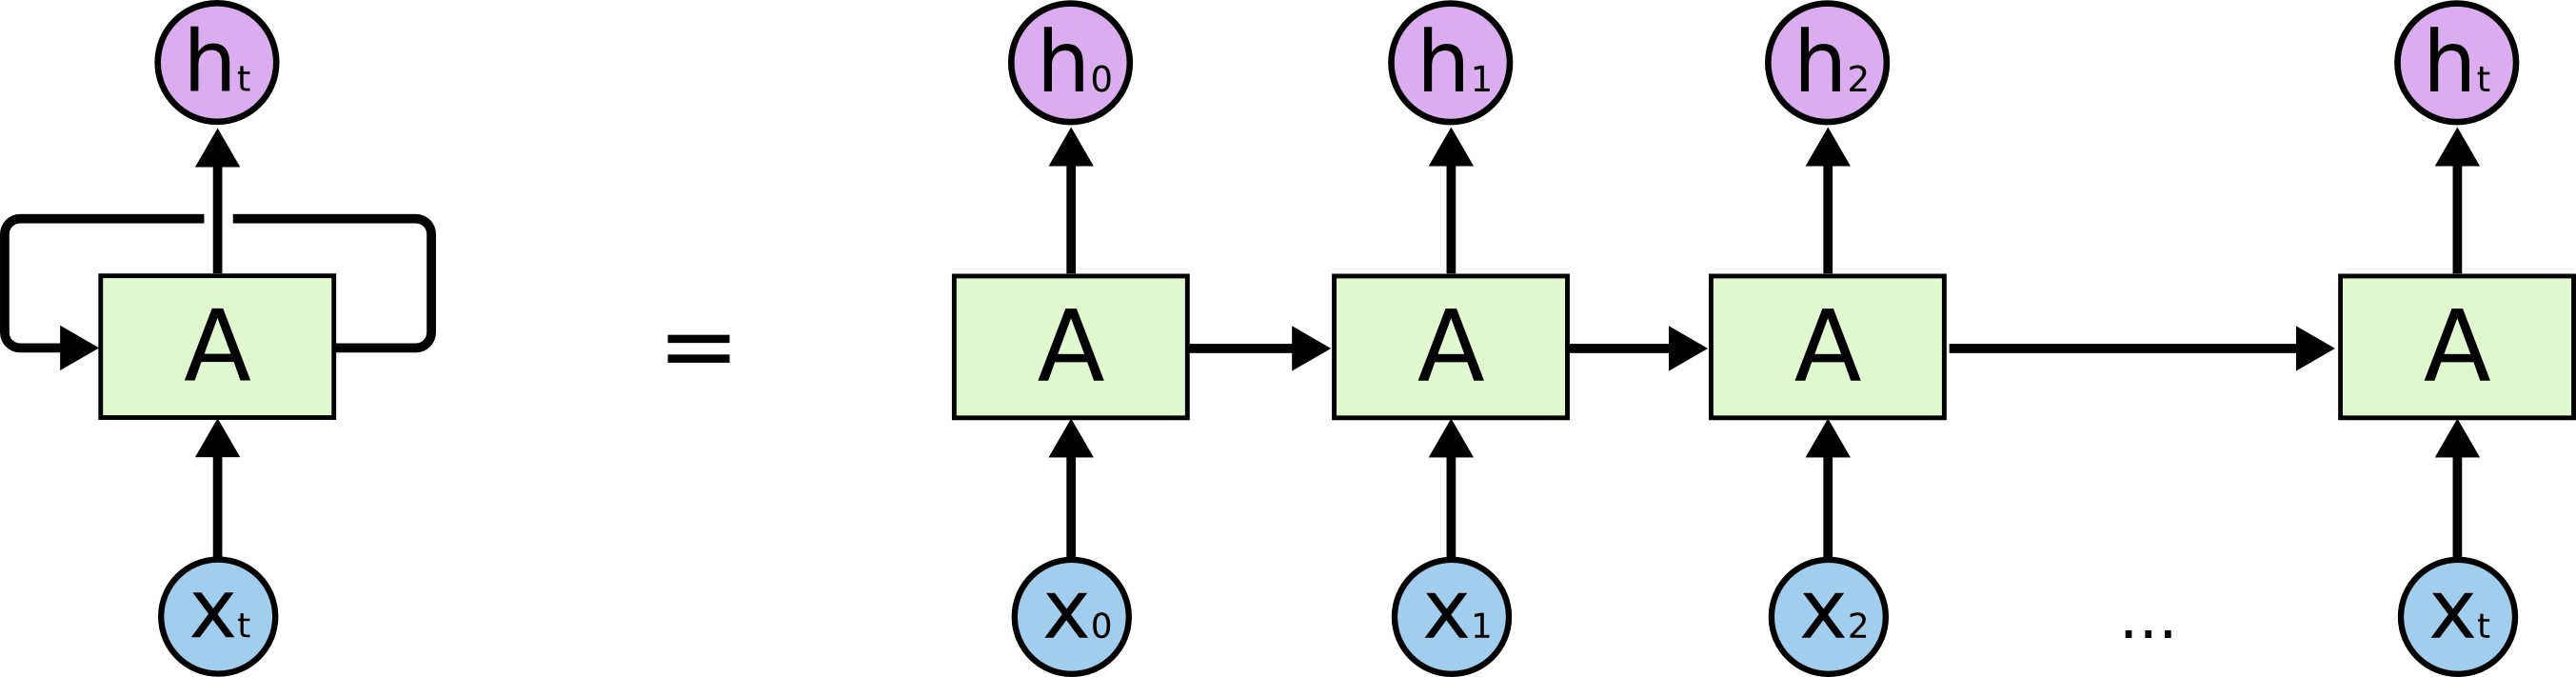
\includegraphics[width=0.9\linewidth]{LSTM/RNN-unrolled}
			\caption[Unfolding the RNN]
			{Unfolding the RNN. Left: The RNN as a cyclic graph. 
				Right: Unfolded RNN for a number of timesteps.
				\imagecourtesycolah}
			\label{fig:RNN-unrolled}
		\end{figure}
		Figure~\ref{fig:RNN-unrolled} shows the RNN as a looping component.
		When unfolded, one can see the information flow from one state to the next.
		Note that it is possible to feed arbitrary sizes of sequences to the RNN.
		
		The simplest implementation of an RNN uses an affine transformation followed by a non-linear function:
		\begin{equation}
			\vectr{h}_t = 
			\tanh \left(
			\matr{W}
			\begin{bmatrix}
				\vectr{x}_t \\
				\vectr{h}_{t-1}
			\end{bmatrix}
			+ \vectr{b}
			\right)
		\end{equation}
		The weight matrix $\matr{W}$ has dimensions $d \times (n + d)$.
		Sometimes it is desirable to have an output that has a different size than the hidden state, e.g., as for classification.
		In this case one can apply a second affine layer
		\begin{equation}
			\vectr{y}_t = \matr{V} \vectr{h}_t + \vectr{c}
		\end{equation}
		to obtain the prediction $\vectr{y}_t$.
		Otherwise we define the output as $\vectr{y}_t = \vectr{h}_t$.
		
		Training an RNN is not much different from a feed-forward network.
		The weights $\vectr{W}, \vectr{V}, \vectr{b}$ and $\vectr{c}$ are updated in the same fashion as for feed-forward networks using gradient descent on the loss function.
		Say we define a criterion $\mathcal{L}_t(\vectr{y}_t, \vectr{\hat{y}}_t)$ for the loss between prediction and ground-truth at each time step $t$.
		Then, the total loss for the sequence is simply 
		\begin{equation}\label{eq:loss_for_rnn}
			\mathcal{L}(\{\vectr{y}_1, \dots \vectr{y}_T\}, \{\vectr{\hat{y}}_1, \dots \vectr{\hat{y}}_T\}) = 
			\sum_{t=1}^{T} \mathcal{L}_t(\vectr{y}_t, \vectr{\hat{y}}_t).
		\end{equation}
		This loss will be used to compute gradients for updating the model parameters similar to feedforward networks.
		
	\section{Gradient Computation for RNNs}\label{sec:gradient_computation_RNN}
		The gradient computation is almost the same as for feed-forward networks and the backpropagation algorithm can be applied by unfolding the RNN as shown in figure~\ref{fig:RNN-unrolled}.
		However, there is a problem with the gradient computation in the above version of the RNN (\cite{pascanu2013difficulty}, \cite{bengio1994learning}).
		For long sequences, the gradient norm can become very small and this hurts the training.
		The RNN is not able to learn long-term dependencies when the gradient vanishes.
		To see this, we can write down the full equation for the gradient:
		\begin{equation}\label{eq:gradient_computation_RNN}
			\frac{\partial \mathcal{L}}{\partial \vectr{w}}
			= \sum_{t=1}^{T} 
				\frac{\partial \mathcal{L}_t}{\partial \vectr{w}}
			= \sum_{t=1}^{T} 
				\sum_{k=1}^{t} 
					\frac{\partial \mathcal{L}_t}{\partial \vectr{y}_t}
					\frac{\partial \vectr{y}_t}{\partial \vectr{h}_t}
					\left(
						\prod_{j=k+1}^{t} \frac{\partial \vectr{h}_j}{\partial \vectr{h}_{j-1}}
					\right)
					\frac{\partial \vectr{h}_{k}}{\partial \vectr{w}}
		\end{equation}
		In the above equation, we have the product term that causes the problem when the sequence is very long.
		Note that the partial derivatives are Jacobian matrices when we take the derivatives of a vector-valued function with respect to a vector.
		Due to many multiplications, the gradient values drop exponentially.
		\todo{Need a better explanation why values are <1 and drop exponentially}
		A more complete analysis is provided in \cite{pascanu2013difficulty}.
		
	\section{The Long Short-Term Memory}
		\begin{figure}[tb]
			\centering
			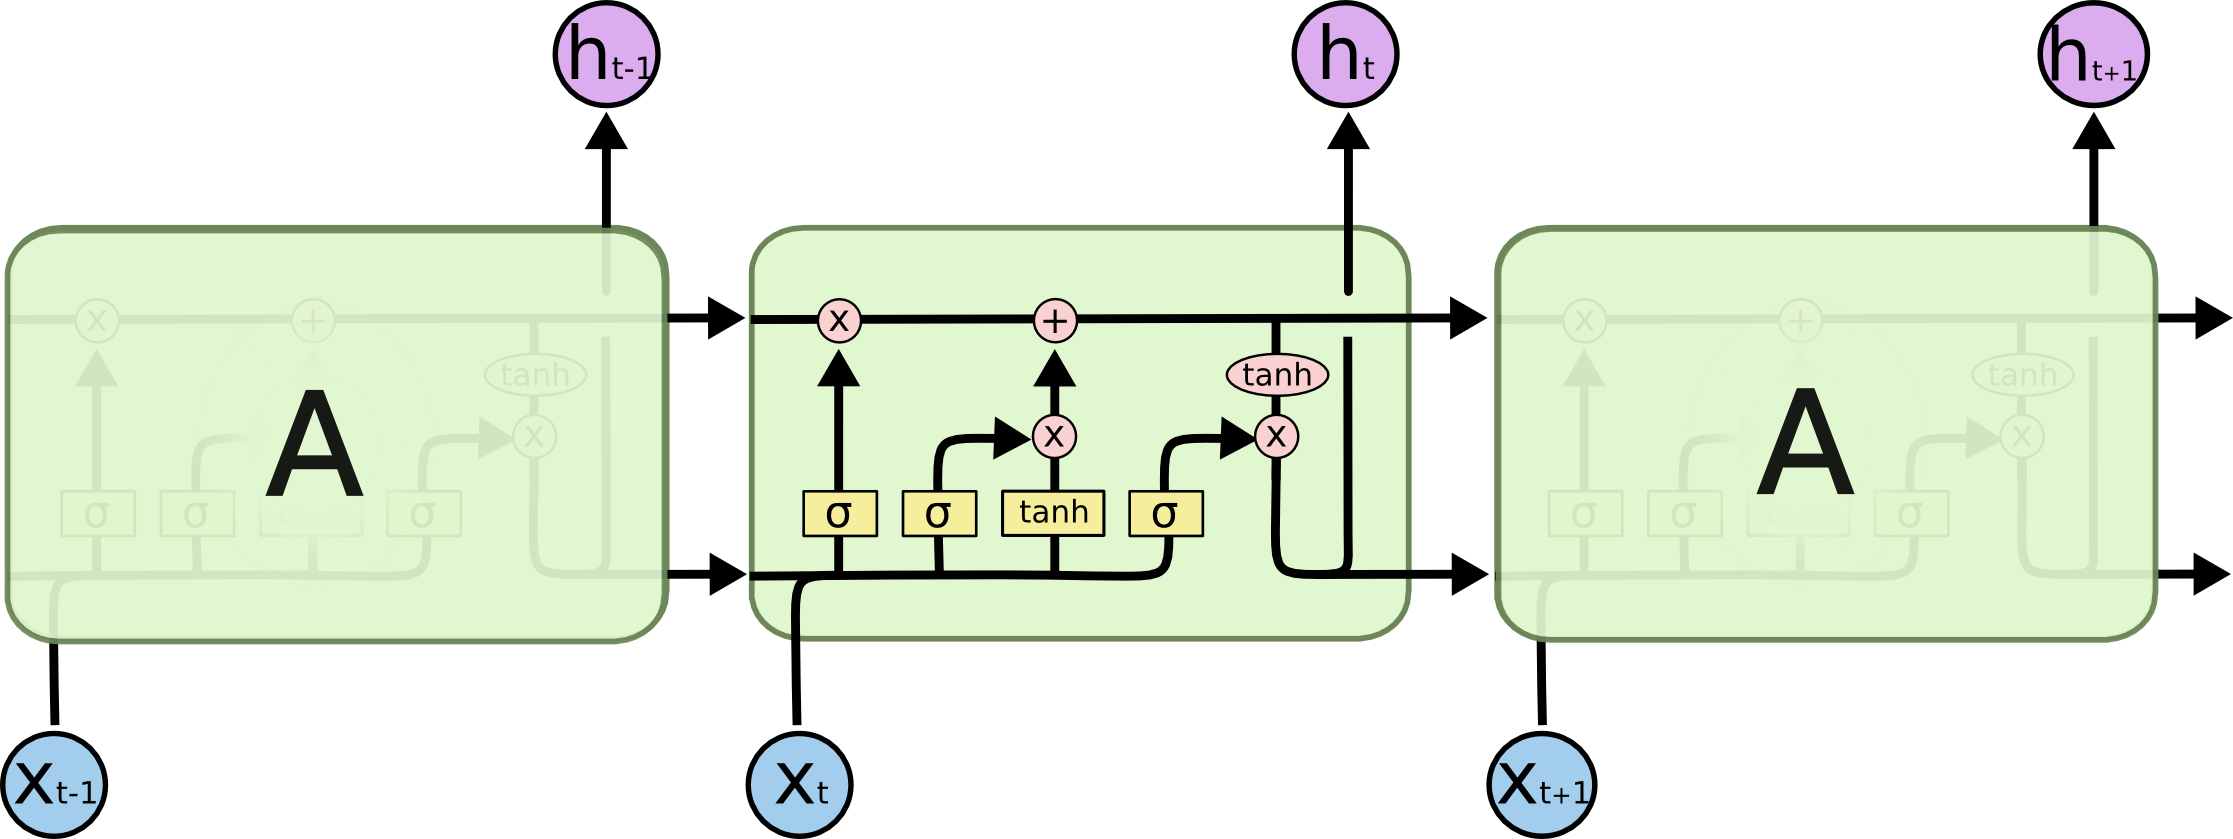
\includegraphics[width=0.9\linewidth]{LSTM/LSTM3-chain}\\
			\vspace{5mm}
			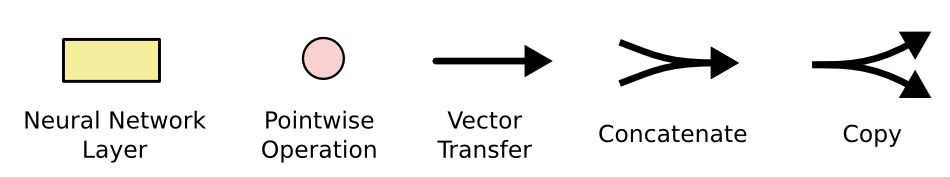
\includegraphics[width=0.5\linewidth]{LSTM/LSTM2-notation}
			\caption[Unfolded LSTM cell]
					{Unfolded LSTM cell. 
					\imagecourtesycolah}
			\label{fig:LSTM3-chain}
		\end{figure}
		The Long Short-Term Memory (LSTM) is a version of the RNN that was designed to overcome the vanishing gradient problem described above, and it is also used in this thesis.
		As shown in figure~\ref{fig:LSTM3-chain}, it introduces four gates (in yellow) and an additional cell state variable that is carried over from one time step to the next.
		The recurrence can be formulated as a function 
		% $R \colon \R^n \times \R^d \times \R^d \rightarrow \R^d \times \R^d$
		\begin{align}\label{eq:LSTM_recurrence}
			(\vectr{h}_t, \vectr{c}_t) = R(\vectr{x}_t, \vectr{h}_{t-1}, \vectr{c}_{t-1}), & & t = 1, \dots, T.
		\end{align}
		More precisely, the hidden state and cell state are computed as follows:
		\begin{align}\label{eq:Vanilla-LSTM-Definition}
			\begin{split}
				\begin{bmatrix}
					\vectr{i} \\ 
					\vectr{f} \\ 
					\vectr{o} \\ 
					\vectr{g}
				\end{bmatrix}
				&=
				\begin{bmatrix}
					\sigma \\ 
					\sigma \\ 
					\sigma \\ 
					\tanh
				\end{bmatrix}
				\left(
				\matr{W}
				\begin{bmatrix}
					\vectr{x}_t \\
					\vectr{h}_{t-1}
				\end{bmatrix}
				+
				\begin{bmatrix}
					\vectr{b}_i \\ 
					\vectr{b}_f \\ 
					\vectr{b}_o \\ 
					\vectr{b}_g
				\end{bmatrix}
				\right)
				\\
				\vectr{c}_t &= \vectr{i} \odot \vectr{g} + \vectr{f} \odot \vectr{c}_{t-1} \\
				\vectr{h}_t &= \vectr{o} \odot \tanh(\vectr{c}_{t})
			\end{split}
		\end{align}
		The matrix $\matr{W} \in \R^{4d \times (n + d)}$ contains the weights for the input- and hidden state transformations before each gate.
		It can be broken down into four parts:
		\begin{align}
			\matr{W} &=
			\begin{bmatrix}
				\vectr{W}_i \\ 
				\vectr{W}_f \\ 
				\vectr{W}_o \\ 
				\vectr{W}_g
			\end{bmatrix}
		\end{align}
		We can see that there are three additional gates that control information flow with a sigmoid activation.
		If the sigmoid output is one, all information is let through, otherwise no information passes the gate. 
		
		The first is the input gate $\vectr{i}$.
		It controls how much information should be collected from the current input and hidden state.
		The second is the forget gate $\vectr{f}$, which will learn what information should be discarded from the previous cell state.
		Finally, the output gate $\vectr{o}$ regulates the amount of information that goes to the output $\vectr{h}_t$.
		
	\section{Training RNNs}
		% Intro: Two parts - optimization algorithm and how inputs/outputs are defined
		
		\paragraph{Optimization Procedure}
		In order to use the loss function to update the model weights, one has to specify an optimization algorithm.

		\todo{connect}
		
		There are several ways an RNN can be trained.
		First of all, one can distinguish the type of input-output relationship for RNNs.
		
		\paragraph{Input to Output Mapping}
		In section~\ref{sec:recurrent_neural_networks} it was assumed that for each time step $t$ there is an input $\vectr{x}_t$ and an output $\vectr{h}_t$.
		This is the most general setup for an RNN and we refer to it as \emph{many-to-many}. 
		
		For some tasks, it might not be suitable to have an input at each time, or an output at each time.
		On the other hand, the RNN is not a feedforward network in the time axis and thus does not allow a modification to remove inputs or outputs at certain time steps.
		However, this does not mean that one has to use all outputs for computing loss and gradients.
		For example, if we wish to predict the sentiment of a sentence, we can feed each word to the RNN and and ignore all outputs except the last one and use that for backpropagation of the gradient.
		We refer to this method as \emph{many-to-one}.
		If there is only one input available, but the output must a sequence (\emph{one-to-many}), one possibility is to simply feed the same input for all time steps.
		An example for this method is image captioning, where the input is an image and the output is a description of the image in form of a sentence. \todo{reference to a work on image captioning}
		Finally, the \emph{one-to-one} setting is a combination of the two above.
		
		\paragraph{Signaling Output} 
		Instead of ignoring certain outputs and only using the ones needed, an alternative is to use a special input symbol $\vectr{e}$ to explicitly signal that an output should be written.
		This special token has to be encoded with the same dimensionality as the other inputs. 
		Its numerical value can be fixed before training (as a hyperparameter) or it can be part of the model parameters and be learned.
		For example, in the sentiment analysis example from before, the token can be used as an end-of-sequence symbol to mark the end of a sentence.
		In general, the symbol does not necessarily have to be used at the end of a sequence.
		It can be inserted whenever an output is needed.
		An application of this is shown in an experiment later in the thesis. 
		\todo{Explicitly refer to the section}
		
		\paragraph{Truncated Backpropagation}
		As discussed in section~\ref{sec:gradient_computation_RNN}, gradient computation over long sequences can cause vanishing or exploding values that hinder the learning process during training.
		The LSTM was designed to addressed this issue, but backpropagation over very long sequences is still computationally expensive.
		As a compromise, one can choose to backpropagate only a certain amount of time steps.
		This is called \emph{truncated backpropagation through time} or TBPTT.
		In order to save memory and reduce computation, one can choose to limit the gradient computation through time.
		This is called \emph{truncated backpropagation through time (TBPTT)}. 
		Say the sequences have a length of $T$ and the number of time steps to backpropagate is $\tau \leq T$.
		To compute the gradient only back to $T - \tau$, we can replace the start indices for $t$ and $k$ in the sums of equation~\ref{eq:gradient_computation_RNN} with $T - \tau$.
		Obviously, this is an approximation of the full gradient over all time steps.
		The RNN is not forced to learn dependencies back in time longer than $\tau$ steps and thus we can not expect it to do so.
		\todo{mention where this is used later in thesis}
		
		A specific application of TBPTT is for training on one continuous data stream instead of many shorter sequences.
		For example, if the goal is to train an RNN to generate natural text, it needs to remember the context over multiple sentences.
		To do this, one can concatenate the data from all text documents to one very long sequence.
		During training, we can forward subsequences consecutively and backpropagate $\tau$ steps.
		After each backpropagation, the hidden state $\vectr{h}_t$ (or $(\vectr{h}_t, \vectr{c}_t)$ in the case of LSTM) is carried over to the next subsequence as initial state.
		This way, there is always information available from the past even though the gradients are never propagated to the very beginning of the sequence.
		\todo{mention where this is used later in thesis}
		
		\paragraph{Ground Truth}
		How ground truth is used depends heavily on the task at hand.
		In the aforementioned example for generating text, the RNN predicts the next word given the current word and the context (hidden state).
		Therefore, the ground truth data is the same as the input data except that it is shifted in time, e.g., $\vectr{y}_t = \vectr{x}_{t + 1}$.
		In this example, not only do the input and output have the same dimensionality (words are encoded as vectors), but the semantic meaning is also the same.
		This is of course not true for all applications of RNNs.
		In this thesis, the inputs are camera images (thousands of color values) and the outputs are poses (usually 6D or 7D vectors).
		The semantic gap is large since the pose is not directly encoded in the individual image, but in the motion between the frames.
		The pose is always relative to the first frame in the sequence.
		The RNN has to learn this directly from the ground truth, not from the input.
		
		
		% How the ground truth is used
		% 	Does ground truth have same dimensionality as input?, as hidden state?
		%
		
	\section{PyTorch}
		PyTorch is a deep learning framework for Python that comes with a rich tensor library.
		It differs from other libraries (TensorFlow, Caffe, Theano and more) in the sense that it builds the computational graph dynamically at runtime.
		This flexibility allows for controlling the computational flow while training or testing the network.
		
		
		
	\section{Exploring the LSTM}
	\todo{Alternative titles: Capabilities of LSTMs, Strengths and Weaknesses of LSTM, Analysis of LSTMs, The LSTM: A Analysis}

		The aim of this chapter is to develop an understanding of how the recurrent neural networks work, specifically the LSTM.
		We begin with a very simple memorization task to demonstrate how an LSTM is trained on sequences of data and what effect different hyperparameters have.
		Building on this knowledge, we explore more sophisticated tasks such as predicting the motion of a cloud of points which will finally lead into the challenging problem of visual odometry and structure from motion.
	
	\section{A First Toy Example: Memorizing Digits}
		% Capabilities of LSTM
		% - Memory: Describe binary memory example (sequence of binary digits)
		% - As classification, formula for cross-entropy loss
		% - All formulas for LSTM (gates etc.)
		% - What is the purpose of Hidden size for remembering sequence
		% - What would one possible solution for the LSTM weights?
		% - 
		
		%To understand how LSTMs are used to learn from sequences of data and how their memory works, we conduct a small example for demonstration. 
		This first experiment is to show the capabilities and limitations of the LSTM.
		Can it memorize the past and use this knowledge for future outputs?
		And how far back in time can it remember?
		Does it work best for classification or regression?
		\todo{Regression still missing from experiments! (one fig. generated)}
		These are the main questions that are investigated in this section.
		
		\paragraph{The Task}
		The goal is to train an LSTM that remembers the last $m$ digits of a random sequence of binary digits $\vectr{x}_t \in \{0, 1\}$. 
		Thus, at time $t$ we would like the output to be the digit $\vectr{x}_{t-m}$ that was fed $m$ time steps before. 
		For example, here are two sequences of zeros and ones shifted by $m = 3$:
		\newcommand{\hlc}[2][yellow]{{%
				\colorlet{foo}{#1}%
				\sethlcolor{foo}\hl{#2}}%
		}
		\begin{center}
			\texttt{\dots01\hlc[pink]{1}\hlc[green!45]{1}\hlc[cyan!50]{0}10110\dots}
			\\
			\texttt{\dots00101\hlc[pink]{1}\hlc[green!45]{1}\hlc[cyan!50]{0}10\dots}
		\end{center}
		The first line is the input sequence and below is the desired output sequence.
		The LSTM reads the digits one by one to store them in memory and at the same time it outputs the digit from memory at time $t - 3$ as highlighted by the colors above.
		%How can we model and train this sequence-to-sequence problem?
		
		In order to tackle a machine learning problem, one needs to define three key elements:
		\begin{enumerate}
			\item Model
			\item Performance measure
			\item Optimization procedure
		\end{enumerate}
	
		\paragraph{The Model}
		We begin by defining the model.
		The first part of our model is the LSTM itself as it was defined in equations~\ref{eq:LSTM_recurrence} and~\ref{eq:Vanilla-LSTM-Definition}.
		Since the output can only be two numbers (zero and one), we will treat the problem as a classification task.
		To do this, we add an affine layer to shrink the size of the LSTM output $\vectr{h}_t$ down to a two-element vector
		\begin{equation}
			\vectr{z}_t = \matr{V} \vectr{h}_t + \vectr{c}.
		\end{equation}
		The last layer is the \emph{softmax} operation
		\begin{eqnarray}
			\text{softmax}(\vectr{x})_j = \frac{e^{x_{j}}}{\sum_{k=1}^{K} e^{x_{k}}},  & & j = 1, \dots, K
		\end{eqnarray}
		which is applied to $\vectr{z}_t$, where $K = 2$ in this example.
		The softmax layer forces the output to be a probability vector, which means that each entry is in the range $[0, 1]$ and all elements sum to one.
		Therefore, the output vector contains two probabilities, 
		\begin{equation*}
			\vectr{p}_t = 
			\begin{bmatrix}
				P(\vectr{o}_t = 0 \mid \vectr{x}_t, \vectr{h}_{t - 1}, \vectr{c}_{t - 1}) \\ 
				P(\vectr{o}_t = 1 \mid \vectr{x}_t, \vectr{h}_{t - 1}, \vectr{c}_{t - 1})
			\end{bmatrix}.
		\end{equation*}
		The output digit $\vectr{o}_t$ must be chosen according to the highest probability.
		A summary of the full model is shown in table~\ref{tbl:model_classification_binary_digits}.
		\begin{table}[tb]
			\small
			\begin{center}
				\begin{tabular}{|l|c|c|c|c|}
					\hline
					Layer 	& Variable 			& Input size 	& Output size 	& Parameters 			\\ \hline
					LSTM 	& $\vectr{h}_t$		& 1 			& $d$ 			& $4d(d + 1) + 4d$ 		\\ \hline
					Affine 	& $\vectr{z}_t$		& $d$ 			& 2 			& $2d + 2$ 				\\ \hline
					Softmax & $\vectr{p}_t$		& 2 			& 2 			& 0						\\ \hline
				\end{tabular}
			\end{center}
			\caption[A simple model to memorize a binary sequence]
					{A simple model to memorize a binary sequence. 
				 The variable $d$ is the hidden size of the LSTM.}
			\label{tbl:model_classification_binary_digits}
		\end{table}
		
		\paragraph{The Performance Measure}
		Next, we have to define a suitable loss function. 
		For classification with softmax as the last layer, it is preferable to use the negative log-likelihood
		\begin{equation}
			\mathcal{L}(\vectr{x}, y) = -\log\left(\vectr{x}_y\right)
		\end{equation}
		as a loss function. 
		Here, the first argument of $\mathcal{L}$ would be replaced with the output $\vectr{p}_t$ of the network and the second argument is the ground truth label. 
		Since we are predicting the digit from $m$ time steps ago, the ground truth directly comes from the input sequence, and therefore the label $y_t$ at time $t$ is the input $\vectr{x}_{t - m}$.
		By minimizing this loss, the probability for the correct class is maximized.
		As described in equation~\ref{eq:loss_for_rnn}, the total loss for the entire sequence is the sum over the individual losses.
		\todo{need better explanation of log-likelihood loss here}
		
		\paragraph{The Optimization Procedure}
		\todo{rework this paragraph}
		In order to use the loss function to update the model weights, one has to specify an optimization algorithm.

		
		Because this experiment is completely artificial, it is possible to generate as much data as needed.
		Instead of generating many smaller sequences, one can generate a single large sequence or sample the digits on-the-fly.
		In order to save memory and reduce computation, one can choose to limit the gradient computation through time.
		This is called \emph{truncated backpropagation through time (TBPTT)}. 
		Starting from the beginning of the sequence, $T$ inputs are fed to the LSTM followed by the loss computation.
		The gradient computation is performed for exactly $T$ steps back in time and the weights are updated accordingly. 
		Continuing with this pattern, the next $T$ inputs are fed for the next update and so on.
		In each step, the hidden state is carried over from the previous digit.
		This way, there is always information available from the past even though the gradients are never propagated to the very beginning of the sequence.
		\todo{Explain this in the theoretical section, also explain how (truncated) backpropagation works for LSTM}
		
		\paragraph{Results for Binary Sequence}
		Now that task, model and optimization procedure are defined, the model can be trained and evaluated.
		For all experiments, we train the model and test on new unseen data of the same size by computing the accuracy, that is the relative frequency of correctly predicted digits.
		First, let's train and evaluate on the simplest model possible: The LSTM has a hidden size of one ($d = 1$).
		\begin{figure}[tb]
			\centering
			\begin{subfigure}[b]{0.5\linewidth}
				\centering
				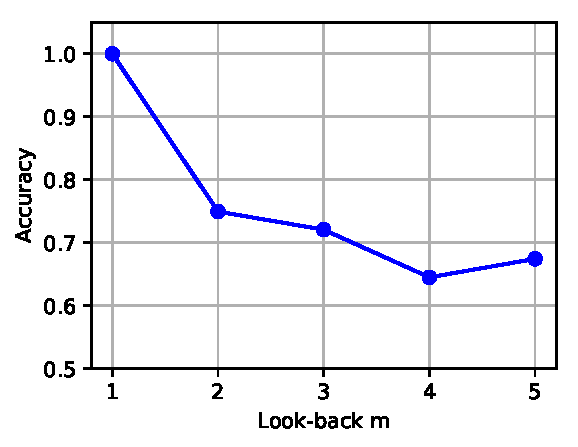
\includegraphics[width=\linewidth]{Python-Plots/memory/accuracy-vs-look-back}
				\caption{
					$d = 1, T = 50, \lambda = 0.01, N = 10^5$
					\label{fig:accuracy-vs-look-back}
				}
			\end{subfigure}%
			\begin{subfigure}[b]{0.5\linewidth}
				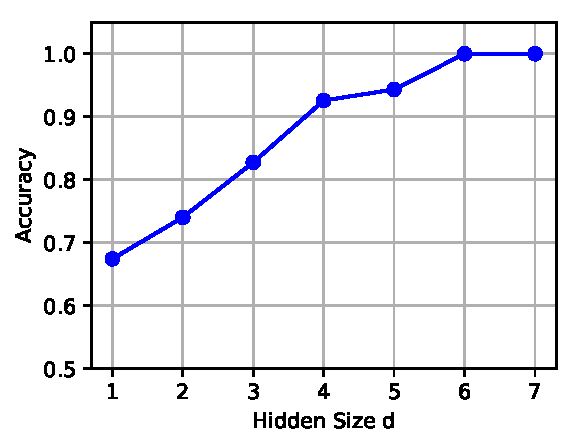
\includegraphics[width=\linewidth]{Python-Plots/memory/accuracy-vs-hidden-size}
				\caption{
					$m = 5, T = 50, \lambda = 0.01, N = 10^5$
					\label{fig:accuracy-vs-hidden-size}
				}
			\end{subfigure}
			\\
			\begin{subfigure}[b]{0.5\linewidth}
				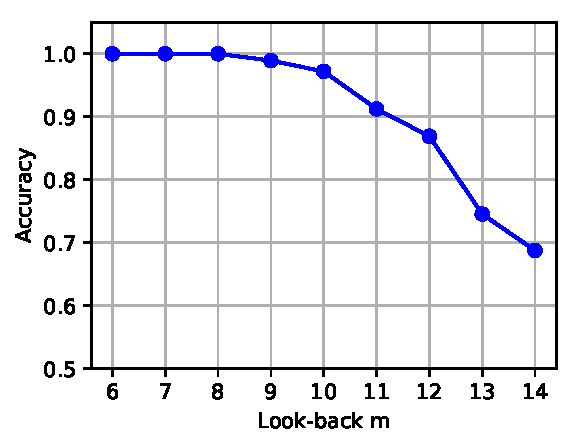
\includegraphics[width=\linewidth]{Python-Plots/memory/accuracy-vs-look-back2}
				\caption{
					$d = 50, T = 50, \lambda = 0.001, N = 10^5$
					\label{fig:accuracy-vs-look-back2}
				}
			\end{subfigure}%
			\begin{subfigure}[b]{0.5\linewidth}
				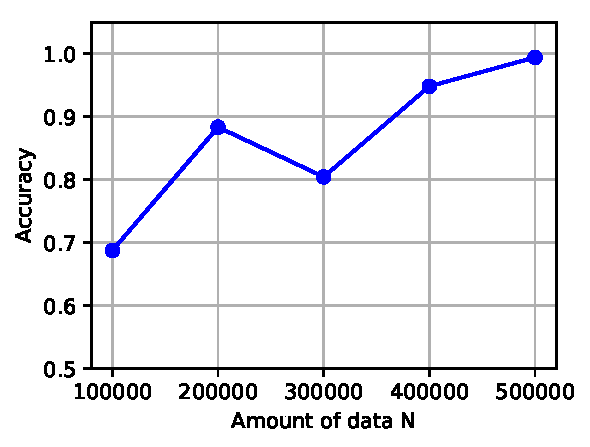
\includegraphics[width=\linewidth]{Python-Plots/memory/more-training-data}
				\caption{
					$m = 14, d = 50, T = 50, \lambda = 0.001$
					\label{fig:more-training-data}
				}
			\end{subfigure}
			\caption[Memorizing the past with the LSTM: Binary digits]
			{Accuracy on the test dataset for varying parameters while keeping others fixed. 
				The parameters involved are the hidden size $d$, look-back $m$, BPTT $T$, training set size $N$ and learning rate $\lambda$. 
				(a) The hidden size is too small.
				(b) Effect of increasing the hidden size.
				(c) Only increasing the hidden size is not enough.
				(d) Increasing the amount of training data.}
			\label{fig:ablation-study-binary-memory}
		\end{figure}
		The result is shown in figure~\ref{fig:accuracy-vs-look-back}. 
		We observe that the model can perfectly memorize the digit of one time step in the past ($m = 1$).
		However, when increasing the look-back the accuracy drops significantly.
		This problem can be fixed by increasing the hidden size as shown in~\ref{fig:accuracy-vs-hidden-size}.
		Based on these observations, it seems that the hidden size $d$ is related to the memory capacity of the network and must always be chosen higher than the look-back $m$. 
		But this hypothesis does not hold true when we continue to increase $m$ as demonstrated in~\ref{fig:accuracy-vs-look-back2}.
		Figure~\ref{fig:more-training-data} shows that for higher look-back, we also need significantly more training data. 
		
		\paragraph{Extension to Multi-class}
		So far we have learned a binary classifier, but we can extend the task to go beyond that to make the problem harder.
		Instead of having only two symbols 0 and 1, we can choose each digit to be a number $\vectr{x}_t \in \{1, \dots, C\}$.
		This is essentially a classification problem with $C$ classes.
		The updated model is shown in table~\ref{tbl:model_classification_multi_class_digits}.
		\begin{table}[tb]
			\small
			\begin{center}
				\begin{tabular}{|l|c|c|c|c|}
					\hline
					Layer 	& Variable 			& Input size 	& Output size 	& Parameters 			\\ \hline
					LSTM 	& $\vectr{h}_t$		& 1 			& $d$ 			& $4d(d + 1) + 4d$ 		\\ \hline
					Affine 	& $\vectr{z}_t$		& $d$ 			& $C$ 			& $Cd + C$ 				\\ \hline
					Softmax & $\vectr{p}_t$		& $C$ 			& $C$ 			& 0						\\ \hline
				\end{tabular}
			\end{center}
			\caption[A simple model to memorize a sequence of numbers]
					{A simple model to memorize a sequence of numbers.
				 This is a generalization of the binary model in table~\ref{tbl:model_classification_binary_digits} where $C = 2$.}
			\label{tbl:model_classification_multi_class_digits}
		\end{table}
		The model is trained and evaluated for each value $C \in \{1, \dots 15\}$.
		\begin{figure}[tb]
			\centering
			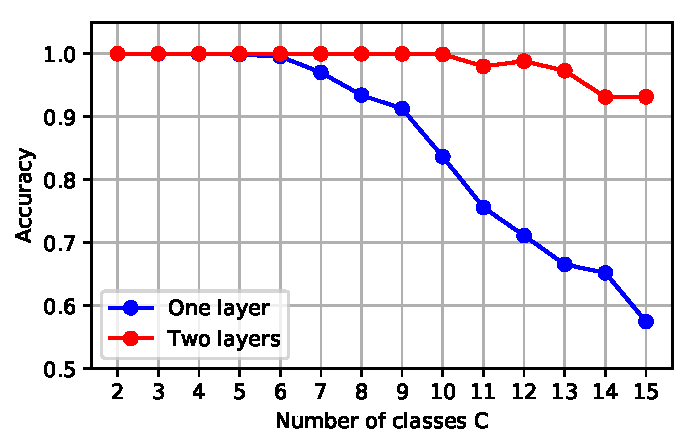
\includegraphics[width=0.7\linewidth]{Python-Plots/memory/accuracy-vs-multiple-classes-and-layers}
			\caption[Memorizing the past with the LSTM: Multiple classes]
					{Memorizing multiple classes with LSTM.
				 Performance of single layer LSTM vs. stacked LSTM.
				 Adding more layers helps deal with the higher complexity of the output.
				 Hyperparameters: $m = 5, d = 50, T = 50, \lambda = 0.001, N = 10^5$.
				 }
			\label{fig:accuracy-vs-multiple-classes-and-layers}
		\end{figure}
		The blue line in figure~\ref{fig:accuracy-vs-multiple-classes-and-layers} shows that the accuracy decreases the more classes are used in the sequence.
		This is due to the more complex mapping between input and output. 
		An LSTM with a single layer can not handle the complexity.
		As shown in the red line in figure~\ref{fig:accuracy-vs-multiple-classes-and-layers}, adding a second layer boosts the performance.
		
		
	\section{Tracking a Moving Point Cloud}
		
		Up to this point, the input to the LSTM was always one-dimensional (a number/digit).
		But how well can it handle vectors as input?
		This is the main question for this section.
		To explore it, we conduct a synthetic experiment for a moving camera.
		
		\paragraph{The Task}
		In this next experiment we would like to study the capabilities of the LSTM on a task for motion estimation.
		To do so, we generate a few 3D points and project them into the image plane of a moving camera.
		This will create an animation of a set of 2D points.
		
		\begin{figure}[tb]
			\centering
			\includegraphics[width=0.7\linewidth]{example-image-a}
			\caption[]
					{\todo{point cloud example, show few points and multiple points}}
			\label{}
		\end{figure}
	
		\paragraph{The Data}
		Each sample from the dataset is a synthetic sequence of frames seen by a moving camera in front of a cloud of 3D points.
		There are two main steps involved in generating the data.
		First, we generate the 3D points.
		Second, the points need to be projected to the screen of each camera.
		The camera is moving left and right to create a simple motion.
		To create a large and diverse dataset, we can generate many such sequences for different point clouds and horizontal motions.
		
		To make this experiment very simple, the points are distributed uniformly on the surface of a sphere.
		This can be done by sampling two random variables $z \sim \mathcal{U}(-1, 1)$ and $\theta \sim \mathcal{U}(0, 2\pi)$ that can be used to parameterize the point
		\begin{equation}
			\vectr{p} = 
			\begin{bmatrix}
				\sqrt{1 - z^2} \cos(\theta) \\ 
				\sqrt{1 - z^2} \sin(\theta) \\
				z
			\end{bmatrix}
		\end{equation}
		on the unit sphere. 
		After repeating this $M$ times, we obtain a cloud $C = \{\vectr{p}_1, \dots \vectr{p}_M\}$ with $M$ points.
		Each of these points has to be projected
		
		
		\paragraph{The Model}
		
		\paragraph{The Optimization Procedure}
		
		\paragraph{Results}
		
		\paragraph{}
	